\documentclass[10pt,aspectratio=169]{beamer}

% silence some Metropolis warnings
\usepackage{silence}
\WarningFilter{beamerthememetropolis}{You need to compile with XeLaTeX or LuaLaTeX}
\WarningFilter{latexfont}{Font shape}
\WarningFilter{latexfont}{Some font}

% define custom colors
\usepackage{xcolor}
\definecolor{dark gray}{HTML}{444444}
\definecolor{light gray}{HTML}{777777}
\definecolor{dark red}{HTML}{BB0000}
\definecolor{dark green}{HTML}{00BB00}
\definecolor{RoyalBlue}{cmyk}{1, 0.50, 0, 0}

% configure metropolis
\usetheme[numbering=fraction]{metropolis}
\setbeamercolor{background canvas}{bg=white}
\setbeamercolor{frametitle}{bg=dark gray}
\setbeamercolor{alerted text}{fg=dark red}
\setbeamercolor{item projected}{bg=dark red}
\setbeamercolor{local structure}{fg=dark red}
\setbeamersize{text margin left=0.5cm,text margin right=0.5cm}
\setbeamercovered{transparent=10}

% use thicker lines
\makeatletter
\setlength{\metropolis@titleseparator@linewidth}{1pt}
\setlength{\metropolis@progressonsectionpage@linewidth}{1pt}
\makeatother

% custom bullet points
\setbeamertemplate{itemize item}{\color{dark red}$\blacktriangleright$}
\setbeamertemplate{itemize subitem}{\color{dark red}$\blacktriangleright$}
\setbeamertemplate{itemize subsubitem}{\color{dark red}$\blacktriangleright$}
\newcommand{\custombullet}{{\color{dark red}$\blacktriangleright$}\hspace{0.5em}}


% imports
\usepackage[english]{babel}
\usepackage[utf8]{inputenc}
\usepackage{amsthm}
\usepackage{amssymb}
\usepackage{amsmath}
\usepackage{amsfonts}
\usepackage{mathtools}
\usepackage{mathabx}
\usepackage{stmaryrd}
\usepackage{graphicx}
\usepackage{hyperref}
\usepackage{xfrac}
\usepackage{appendixnumberbeamer}
\usepackage{tabularx}
\usepackage{listings}

% for code formatting
   \lstset{language=R,
           basicstyle=\ttfamily\scriptsize,
           keywordstyle=\color{blue}\ttfamily,
           stringstyle=\color{red}\ttfamily,
           commentstyle=\color{green}\ttfamily,
          breaklines=true
          }



% check and x marks
\usepackage{pifont}
\newcommand{\cmark}{{\color{dark green}\ding{51}}\hspace{0.3em}}
\newcommand{\xmark}{{\color{dark red}\ding{55}}\hspace{0.5em}}


% use classic font for math
\usepackage[T1]{fontenc} % Needed for Type1 Concrete \usepackage{concmath}
\usefonttheme{serif}
\usefonttheme{professionalfonts}
\usepackage{concmath}
\setbeamerfont{equation}{size=\tiny}



% diagrams
\usepackage{tikz}
\usetikzlibrary{decorations.pathreplacing, arrows, shapes, patterns, angles, quotes}

% references
\usepackage[natbibapa]{apacite}
\bibliographystyle{apacite}
\renewcommand{\bibsection}{}

% use ampersands instead of "and" for text citations
\AtBeginDocument{\renewcommand{\BBAB}{\&}}

% possessive cites
\makeatletter
\patchcmd{\NAT@test}{\else \NAT@nm}{\else \NAT@nmfmt{\NAT@nm}}{}{}
\DeclareRobustCommand\citepos
  {\begingroup
   \let\NAT@nmfmt\NAT@posfmt
   \NAT@swafalse\let\NAT@ctype\z@\NAT@partrue
   \@ifstar{\NAT@fulltrue\NAT@citetp}{\NAT@fullfalse\NAT@citetp}}
\let\NAT@orig@nmfmt\NAT@nmfmt
\def\NAT@posfmt#1{\NAT@orig@nmfmt{#1's}}
\makeatother

% spaced-out lists
\newenvironment{wideitemize}{\itemize\addtolength{\itemsep}{10pt}}{\enditemize}
\newenvironment{wideenumerate}{\enumerate\addtolength{\itemsep}{10pt}}{\endenumerate}

% replace footnotes with buttons
\usepackage[absolute,overlay]{textpos}
\newcounter{beamerpausessave}
\newcommand{\always}[1]{
    \setcounter{beamerpausessave}{\value{beamerpauses}}
    \setcounter{beamerpauses}{0}
    \pause
    #1 
    \setcounter{beamerpauses}{\value{beamerpausessave}}
    \addtocounter{beamerpauses}{-1}
    \pause
}
\newcommand{\buttons}[1]{\always{
    \begin{textblock*}{\paperwidth}(0.015\textwidth, 1.022\textheight)
        \scriptsize
        #1
    \end{textblock*}
}}
\newcommand{\appendixbuttons}[1]{\always{
    \begin{textblock*}{\paperwidth}(0.015\textwidth, 1.043\textheight)
        \scriptsize
        #1
    \end{textblock*}
}}
\newcommand{\goto}[2]{\hyperlink{#1}{{\color{dark red}$\smalltriangleright$} #2}\hspace{0.5em}}
\newcommand{\goback}[2]{\hyperlink{#1}{{\color{dark red}$\smalltriangleleft$} #2}\hspace{0.5em}}

% custom appendix
\renewcommand{\appendixname}{\texorpdfstring{\translate{Appendix}}{Appendix}}

% change color of cites and URLs
\let\oldcite\cite
\let\oldcitet\citet
\let\oldcitep\citep
\let\oldcitepos\citepos
\let\oldcitetalias\citetalias
\let\oldcitepalias\citepalias
\let\oldurl\url
\def\cite#1#{\citeaux{#1}}
\def\citet#1#{\citetaux{#1}}
\def\citep#1#{\citepaux{#1}}
\def\citepos#1#{\citeposaux{#1}}
\def\citetalias#1#{\citetaliasaux{#1}}
\def\citepalias#1#{\citepaliasaux{#1}}
\def\url#1#{\urlaux{#1}}
\newcommand*\citeaux[2]{{\color{light gray}\oldcite#1{#2}}}
\newcommand*\citetaux[2]{{\color{light gray}\oldcitet#1{#2}}}
\newcommand*\citepaux[2]{{\color{light gray}\oldcitep#1{#2}}}
\newcommand*\urlaux[2]{{\color{light gray}\oldurl#1{#2}}}
\newcommand*\citeposaux[2]{{\color{light gray}\oldcitepos#1{#2}}}
\newcommand*\citetaliasaux[2]{{\color{light gray}\oldcitetalias#1{#2}}}
\newcommand*\citepaliasaux[2]{{\color{light gray}\oldcitepalias#1{#2}}}

% custom math commands
\DeclareMathOperator*{\argmax}{argmax}
\DeclareMathOperator*{\argmin}{argmin}
\renewcommand{\Pr}{\mathbb{P}}
\newcommand{\E}{\mathbb{E}}
\newcommand{\Var}{\mathbb{V}}
\newcommand{\Cov}{\mathbb{C}}
\newcommand{\overbar}[1]{\mkern 1.5mu\overline{\mkern-1.5mu#1\mkern-1.5mu}\mkern 1.5mu}
\newcommand{\abs}[1]{\lvert#1\rvert}
\newcommand{\norm}[1]{\lVert#1\rVert}

% tables
\usepackage{booktabs}
\usepackage{colortbl}
\usepackage{multirow}
\usepackage{makecell}
\arrayrulecolor{dark red}

% custom date
\usepackage{datetime}
\newdateformat{monthyeardate}{\monthname[\THEMONTH] \THEYEAR}

% fix pauses with graphics
\usepackage{../resources/fixpauseincludegraphics}


\begin{document}

\pgfmathdeclarefunction{gauss}{2}{%
  \pgfmathparse{1/(#2*sqrt(2*pi))*exp(-((x-#1)^2)/(2*#2^2))}%
}

\title{Econometrics I}
\subtitle{Lecture 1: Probability}

\author{Chris Conlon \\NYU Stern}
\date{Fall 2025}
\maketitle


\begin{frame}{Roadmap}
\begin{enumerate}
	\item Probability spaces
	\item Random variables
	\item Distribution and density functions
	\item Moments of random variables, mean and variance
	\item Conditional expectations
	\item Multivariate distributions
	\item Independence
	\item Bayes's Theorem
	\item Law of Iterated Expectations
\end{enumerate}
\end{frame}



\begin{frame}{Basic Definitions}
To discuss probability we first need a few basic definitions:
\begin{itemize}
	\item An {\bf outcome} is something we \emph{can} observe but may not know in advance
	\begin{itemize}
		\item[] \emph{Example:} For a coin flip, $H$ (heads) is an outcome
		\item[] \emph{Example:} The wage of a randomly sampled worker
	\end{itemize}	
	\item A {\bf sample space}, $\Omega$, is a set of all possible outcomes
		\begin{itemize}
		\item[] \emph{Example:} For a coin flip, $\{H,T\}$ is the sample space
		\item[] \emph{Example:} For two coin flips, $\{HH,HT,TH,TT\}$ is the sample space
	\end{itemize}
	\item An {\bf event} is any subset of the sample space
		\begin{itemize}
			\item[] \emph{Example:} For two coin flips, $\{HH,TT\}$ is the event ``getting the same side both times"
		\end{itemize}
		
	\item A {\bf probability} is a function from $S$, the set of all events, to $[0,1]$ such that
	{\small \begin{enumerate}
			\item $P(E)\in[0,1]$ for any event, $E$
			\item $P(\Omega)=1$
			\item $P(A\cup B) = P(A)+P(B)$ whenever $A\cap B = \emptyset$
		\end{enumerate}}

\end{itemize}
\end{frame}




\begin{frame}{Outcomes and Events as a Venn Diagram}


\def\firstcircle{(0,0) circle (1.5cm)}
\def\secondcircle{(0:2cm) circle (1.5cm)}

% Now we can draw the sets:
\begin{figure}
	\centering
\begin{tikzpicture}
	\draw (-2,-2.5) rectangle (4,2.5);
    \draw[fill = blue, fill opacity=.2] \firstcircle;
    \draw[fill = red, fill opacity=.2] \secondcircle;
    \node(A) at (0,0){\small $A$};
    \node(AB) at (1,0){\small $A\cap B$};
    \node(B) at (2,0){\small $B$};
    \node(S) at (3.5,2){\small $\Omega$};
    
    % A intersect B
%    \begin{scope}
%      \clip \firstcircle;
%      \fill[color = red,fill opacity=0.2] \secondcircle;
%    \end{scope}
%    
%    % A intersect B intersect C
%    \begin{scope}
%      \clip \firstcircle;
%      \clip \secondcircle;
%      \fill[color = green, fill opacity=0.2] \thirdcircle;
%    \end{scope}
%    
%    \begin{scope}
%    	\clip \firstcircle;
%    	\fill[color = blue, fill opacity=0.2] \thirdcircle;	
%    \end{scope}
\end{tikzpicture}
\end{figure}
\begin{itemize}
	\item $A$ and $B$ are events in the sample space, $\Omega$
	\item The intersection, $A\cap B$, is the purple part	
	\item The union, $A\cup B$, would be everything that isn't white
\end{itemize}


\end{frame}


\begin{frame}{Random Variables}
\begin{itemize}
	\item A random variable assigns numeric values to outcomes:\[
		X:\Omega \rightarrow \mathbb{R}
	\]

	\item We can define a probability distribution on this random variable in terms of our original probability space:	\[
				\Pr(X=x) = \Pr\left(\bigcup_{\omega:X(\omega)=x} \omega\right)
			\]
			
	\item \emph{Example:} If rolling two dice, probability of the sum being 11 is given by:
\begin{align*}	
P(D_1+D_2 = 11) &= P((D_1=5, D_2=6) \cup (D_1=6, D_2=5)) =\\
 &= P(D_1=5, D_2=6) + P(D_1=6, D_2=5)) \\
 &= 1/36 + 1/36 = 1/18
\end{align*}
\end{itemize}
\end{frame}

\begin{frame}{Continuous Random Variables}
\begin{itemize}
	\item For a continuous random variable $X$ the probability that $X=x$ is ``0" since any one outcome happens with vanishingly small probability
	\item Instead we think about \emph{sets} like $\Pr(a<X<b)$
	\item Define the {\bf Cumulative Distribution Function} of $X$ to be:
		\[
			F(x) = \Pr(\omega: X\left(\omega\right) \leq x)
		\]
	\item {\bf n.b.}: CDF's are always weakly increasing and live in $\left[0,1\right]$
	\item Actually, any non-decreasing, right-continuous function $F$ with $\lim_{x\rightarrow-\infty}F\left(x\right)=0$ and $\lim_{x\rightarrow\infty}F\left(x\right)=1$ 
	 	is a CDF.
\end{itemize}
\end{frame}

\begin{frame}[fragile]{Standard Normal (Gaussian) CDF}
\begin{columns}
\begin{column}{0.5\textwidth}
\begin{center}
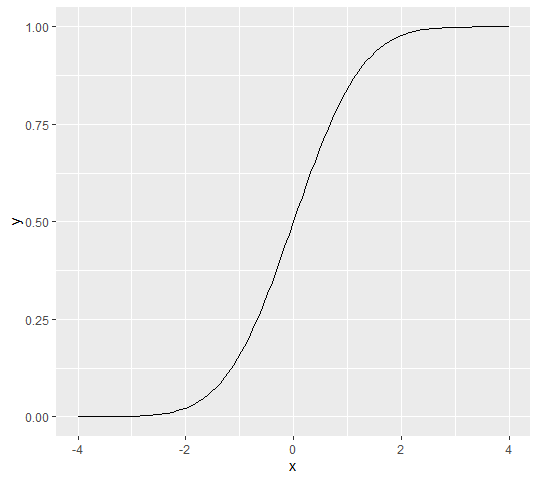
\includegraphics[height=.5\textheight]{normal-cdf} 
\end{center}
\end{column}
\begin{column}{0.5\textwidth} 
\begin{lstlisting}
if(!(require(ggplot2))){install.packages('ggplot2')}
ggplot(data.frame(x = c(-4, 4)), aes(x = x)) +
stat_function(fun = pnorm) +
ylab("cdf") +
ggtitle("Standard Normal CDF") 
\end{lstlisting}
\end{column}
\end{columns}
\[
F\left(x\right) = \frac{1}{2} \left[ 1 + \text{erf}\left(\frac{x-\mu}{\sigma \sqrt{2}} \right)\right]
\]
{\bf n.b.}: $\mu=0$, $\sigma=1$, plotted here, is what we call the {\bf standard} normal
\end{frame}




\begin{frame}[fragile]{Exponential CDF}
\begin{columns}
\begin{column}{0.5\textwidth}
\begin{center}
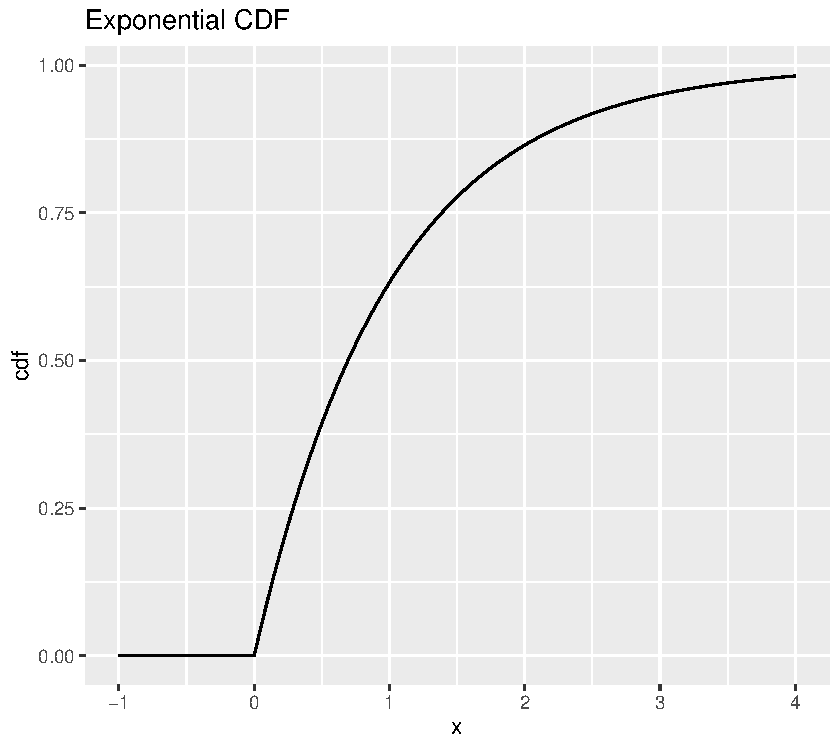
\includegraphics[height=.5\textheight]{exp-cdf} 
\end{center}
\end{column}
\begin{column}{0.5\textwidth} 
\begin{lstlisting}
if(!(require(ggplot2))){install.packages('ggplot2')}
ggplot(data.frame(x = c(-1, 4)), aes(x = x)) +
stat_function(fun = pexp) +
ylab("cdf") +
ggtitle("Exponential CDF")
\end{lstlisting}
\end{column}
\end{columns}
\[
F\left(x\right) = \begin{cases}
	0 & \text{ if }x<0\\
	1 - e^{- \lambda x}  & \text{ if }x\ge 0
\end{cases}
\]
where $\lambda > 0$ is the rate parameter, plotted here for $\lambda=1$.

\end{frame}


\begin{frame}{Check properties of exponential CDF}

\end{frame}



\begin{frame}[fragile]{Bernoulli CDF}
\begin{columns}
\begin{column}{0.5\textwidth}
\begin{center}
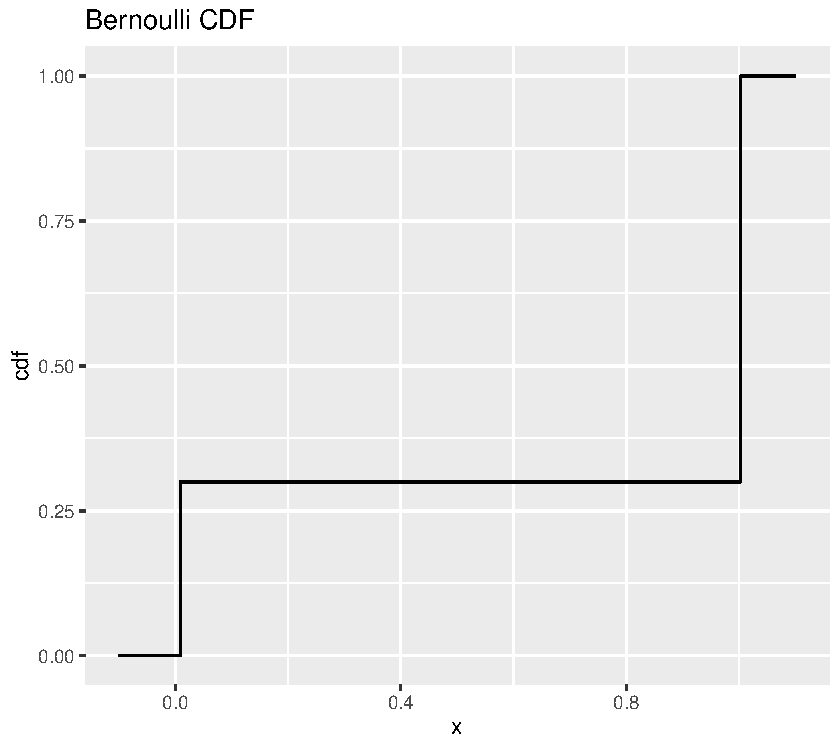
\includegraphics[height=.5\textheight]{bernoulli-cdf} 
\end{center}
\end{column}
\begin{column}{0.5\textwidth} 
\begin{lstlisting}
if(!(require(ggplot2))){install.packages('ggplot2')}
sfun0  <- stepfun(0:1, c(0., .3, 1.), f = 0)  
x = seq(-.1, 1.1, length.out = 100)
df = data.frame(x = x, y = sfun0(x))
ggplot(df, aes(x,y)) + geom_step() +
ylab("cdf")  +
ggtitle("Bernoulli CDF")
\end{lstlisting}
\end{column}
\end{columns}
The Bernoulli distribution describes a random variable $X\in \left\{0,1\right\}$. \\
Plotted is Bernoulli distribution with probability of success $\Pr(X=1)=p=.7$

\end{frame}





\begin{frame}{CDF: draw your own!}
\end{frame}




\begin{frame}{Probability Density Functions}
\begin{itemize}
	\item A random variable's {\bf Probability Density Function} is the derivative of its CDF:
		\[
		 	f(x) = \frac{d}{dx}F(x)
		\]
		
	\medskip
	\item PDFs are well-defined when the CDF is {\bf absolutely continuous} (which requires continuity and almost-everywhere differentiability)
\end{itemize}
\end{frame}



\begin{frame}[fragile]{Standard Normal (Gaussian) PDF}
\begin{columns}
\begin{column}{0.5\textwidth}
\begin{center}
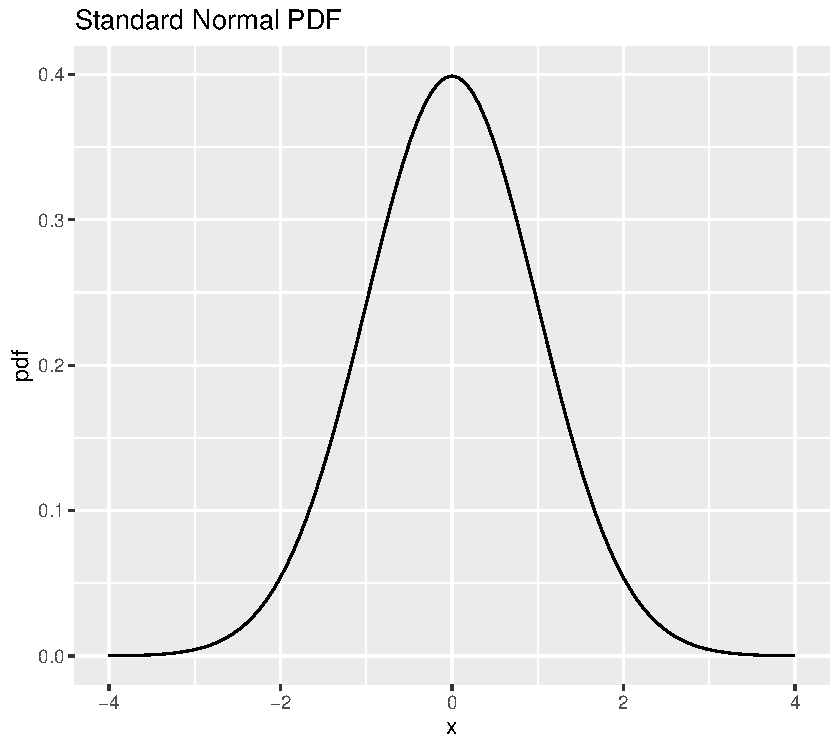
\includegraphics[height=.5\textheight]{normal-pdf} 
\end{center}
\end{column}
\begin{column}{0.5\textwidth} 
\begin{lstlisting}
if(!(require(ggplot2))){install.packages('ggplot2')}
ggplot(data.frame(x = c(-4, 4)), aes(x = x)) +
stat_function(fun = dnorm) + 
ylab("pdf") +
ggtitle("Standard Normal PDF") 
\end{lstlisting}
\end{column}
\end{columns}
\[
f\left(x\right) = \frac{1}{\sigma \sqrt{2 \pi}} \exp\left[ -\frac{1}{2}\left(\frac{x-\mu}{\sigma}\right)^2\right]
\]
{\bf n.b.}: $\mu=0$, $\sigma=1$, plotted here, is what we call the {\bf standard} normal
\end{frame}




\begin{frame}[fragile]{Exponential PDF}
\begin{columns}
\begin{column}{0.5\textwidth}
\begin{center}
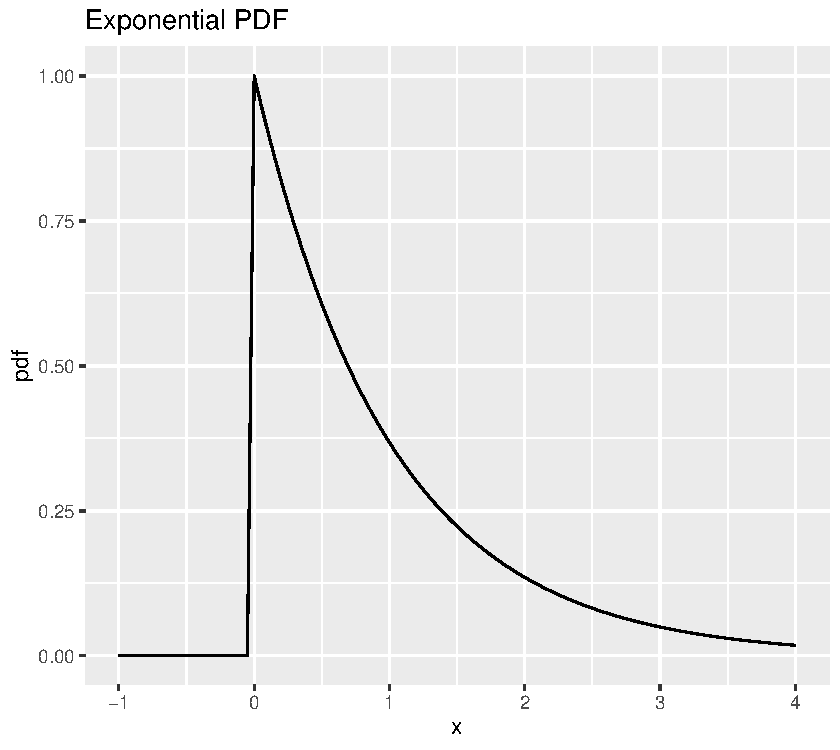
\includegraphics[height=.5\textheight]{exp-pdf} 
\end{center}
\end{column}
\begin{column}{0.5\textwidth} 
\begin{lstlisting}
if(!(require(ggplot2))){install.packages('ggplot2')}
ggplot(data.frame(x = c(-1, 4)), aes(x = x)) +
stat_function(fun = dexp) +
ylab("pdf") +
ggtitle("Exponential PDF")
\end{lstlisting}
\end{column}
\end{columns}
\[
f\left(x\right) = \begin{cases}
	0 & \text{ if }x<0\\
	\lambda e^{- \lambda x} & \text{ if }x\ge 0
\end{cases}
\]
where $\lambda > 0$ is the rate parameter, plotted here for $\lambda=1$.
\end{frame}

\begin{frame}{Discrete vs continuous random variables}
\begin{itemize}
	\item Note that for discrete distributions like the Bernoulli distribution, we
		have discontinuous jumps in the CDF, and the PDF is not defined.
		
	\medskip
	\item Instead of a PDF, we can define a {\bf probability mass function}:
	\[
		p\left(x\right) = \Pr\left(X=x\right)
	\]
	
	\medskip
	\item The set of points $x$ such that $\Pr\left(X=x\right)>0$ are call the {\bf support}
			of $X$. Similarly, the support of a continuously distributed random variable
			can be defined as those points $x$ where the pdf $f(x)>0$.
	
	
		
\end{itemize}
\end{frame}





\begin{frame}{Expectations}
\begin{itemize}
	\item For a continuously distributed random variable:\[
		\E_F \left[ X \right] \equiv \int xf(x)dx
	\]
	
	\medskip
	\item For a discretely distributed random variable:\[
		\E_p \left[ X \right] \equiv \sum_{x\in Supp\left(X\right)} x p\left(x\right)
	\]
	
	\medskip
	\item These expectations are also called the {\bf mean} or {\bf first moment} of $X$. Often, $\mu\equiv \E\left[X\right]$.
		
	\medskip
	\item The $F$ subscript denotes the distribution used to take the expectation. We will often omit it when there is no ambiguity.
\end{itemize}
\end{frame}


\begin{frame}{Expectations of functions of random variables}
\begin{itemize}
	\item For a continuously distributed random variable:\[
		\E_F \left[ g\left(X\right) \right] \equiv \int g\left(x\right)f(x)dx
	\]
	
	\medskip
	\item For a discretely distributed random variable:\[
		\E_p \left[ g\left(X\right) \right] \equiv \sum_{x\in Supp\left(X\right)} g\left(x\right) p\left(x\right)
	\]
	
	\medskip
	\item Note that functions of random variables are random variables themselves, so we're not adding much here.

\end{itemize}
\end{frame}



\begin{frame}{Jensen's Inequality}
\begin{center}
\begin{minipage}{.8\textwidth}
\begin{block}{Jensen's Inequality}
If $g$ is convex, $\E\left[g\left(X\right)\right] \ge g\left(\E\left[X\right]\right)$.

\medskip
If $g$ is concave, $\E\left[g\left(X\right)\right] \le g\left(\E\left[X\right]\right)$.
\end{block}
\end{minipage}
\end{center}
\vspace{0.2cm}
\pause
Application to even moments:
If $g(x)=x^{2 k}$, and $X$ is a random variable, then $g$ is convex as
$$
\frac{d^2 g}{d x^2}(x)=2 k(2 k-1) x^{2 k-2} \geq 0 \quad \forall x \in \mathbb{R}
$$
and so
$$
g(\E[X])=(\E[X])^{2 k} \leq \E\left[X^{2 k}\right]
$$
What does this mean if $k=1$?
\end{frame}


\begin{frame}{Variance}
\begin{itemize}
	\item The variance of a random variable:\[
		Var \left[X\right] \equiv \E\left[\left(X-\mu\right)^2\right]
	\]
	where $\mu=\E\left[X\right]$
	
	\bigskip
	\item Usually, $\sigma^2 \equiv Var \left[X\right] $


	\bigskip
	\item $\E\left[X^k\right]$ is called the {\bf $k$th (uncentered) moment} of $X$
	
	\bigskip
	\item Note that knowing first two moments is equivalent to knowing mean and variance. 
	
\end{itemize}
\end{frame}


\begin{frame}{Pareto distribution}
\begin{itemize}
	\item Pareto distribution:\[
	F\left(x\right)=\begin{cases}
	0 & \text{ if }x<1\\
	1-\left(\frac{1}{x}\right)^{2} & \text{ if }x\ge1
	\end{cases}
	\]

	\medskip
	\item What are the mean and variance of this distribution?
	
\end{itemize}
\end{frame}



\begin{frame}{Moment-generating function}
\begin{itemize}
	\item The moment generating function of $X$ is \[
		m_X \left(t\right) = \E\left[\exp\left(tX\right)\right],
	\]	
	as long as this expectation is defined for $t$ in a neighborhood of zero. 
	
	\medskip 
	\item $\frac{d^k m_X \left(0\right) }{dt^k}$ equals the $k$th moment of $X$.

	\medskip
	\item If two random variables have the same moment generating function, they have the same distribution. [We can use this later].
\end{itemize}
\end{frame}



\begin{frame}{Multivariate distributions}
\begin{itemize}
	\item Econometric models are usually concerned with several random variables.

	\item Denote a {\bf collection} of random variables:\[
		\left\{ X_T\right\}_{t=1}^{T}.
	\]
	Note that $t$ here does not necessarily have anything to do with time.

	\item Examples:
	\begin{itemize}
		\item One of the variables  is ``dependent'' (denoted $Y$) and the others ``explanatory''

		\item A measurement observed repeatedly over time (a {\bf time series}), e.g.,
		\begin{itemize}
			\item the price of a stock
		\end{itemize}

		\item A measurement observed for different individuals (a {\bf cross section}), e.g.,
		\begin{itemize}
			\item wages or income
		\end{itemize}
		\item Most commonly, we will have a combination of these things: multiple observations of several variables. ({\bf panel data})
	\end{itemize}
\end{itemize}
\end{frame}



\begin{frame}{Random vector}
\begin{itemize}
	\item We can now define\[
	{\bf X}_T: \Omega \rightarrow \mathbb{R}^T,
\]
where ${\bf X}_T\left(\omega\right) = \left(X_1\left(\omega\right),\dots,X_T\left(\omega)\right)\right)$
\end{itemize}
\end{frame}



\begin{frame}{Joint and marginal distributions}
\begin{itemize}
\item The {\bf joint} CDF is a natural extension to the CDF for a single random variable:\[
		F_{{\bf X}} \left({\bf x}\right) = \Pr\left(\omega: X_1\left(\omega\right)\le x_1, \dots , X_T\left(\omega\right)\le x_T\right)
	\]
where ${\bf x} = \left(x_1,\dots,x_T\right)\in \mathbb{R}^T$.

\smallskip
\item The {\bf joint PDF} can be defined as $f\left( {\bf x} \right) = \frac{\partial^T F_{{\bf X}} \left({\bf x}\right)}{\partial x_1 \partial x_2 \dots \partial x_T}$.

\smallskip
\item {\bf Marginal distributions} refer to the CDF of the individual $X_t$ variables,\[
		F_{X_t} \left(x\right) = \Pr\left(\omega: X_t\left(\omega\right)\le x \right)
		\]
	Formally, marginal CDFs can be obtained  from joint distributions by integrating
		over the other variables. 


\end{itemize}
\end{frame}


\begin{frame}{Covariance}
\begin{itemize}
	\item Covariance is an important property of the joint distribution of random variables:\[
		Cov\left(X_1,X_2\right) = \E\left[ \left( X_1 - \E\left[X_1\right]\right) \left( X_2 - \E\left[X_2\right]\right)\right]
	\]

	\item And more generally for a random vector\[
		Cov\left({\bf X}_T\right) =\E\left[ \left( {\bf X}_T - \E\left[{\bf X}_T\right]\right) \left( {\bf X}_T - \E\left[{\bf X}_T\right]\right)'\right],
	\]
	which is a $T\times T$ matrix. 

	\item Note that $Cov\left(X,X\right) = Var\left(X\right)$.
\end{itemize}
\end{frame}




\begin{frame}{Properties of expectations and covariance I}
\begin{itemize}
	\item For constants $a,b$, you should be able to show that\[
		\E\left[ a + b X\right] = a + b \cdot \E\left[ X\right] 
	\]

	\medskip
	\item From this, it follows that\[
		Cov\left[ a + b \cdot X_1 , X_2 \right] = b \cdot Cov\left[X_1 , X_2 \right] 
	\]

	\medskip From this, it follows that\[
			Var\left(a + b \cdot X\right) = b^2 \cdot Var\left( X\right) 
	\]
\end{itemize}
\end{frame}


\begin{frame}{Properties of expectations and covariance II}
\begin{itemize}
	\item For constants $a,b$, you should be able to show that\[
		\E\left[ a X + b Y\right] = a  \cdot \E\left[ X\right] + b \cdot \E\left[ Y\right] 
	\]

	\medskip
	\item From this, it follows that\[
		Cov\left[ a X + b Y, Z \right] = a \cdot Cov\left[X , Z\right] + b \cdot Cov\left[Y , Z\right] 
	\]
\end{itemize}
\end{frame}



\begin{frame}{Independence}
\begin{itemize}
	\item Two events $A$, $B \subset \Omega$  are {\bf independent} iff\[
		\Pr\left(A\cap B\right) = \Pr\left( A\right)\, \Pr\left( B\right)
	\]
	
	\medskip
	\item A collection of random variables ${\bf X}$ is {\bf independent} iff\[
		F_{{\bf X}} \left({\bf x}\right) = F_{X_1}\left(x_1\right) F_{X_2}\left(x_2\right) \dots F_{X_T}\left(x_T\right) 
	\]
	
		\medskip
	\item A collection of random variables ${\bf X}$ is {\bf independent} iff for any (measurable) real-valued functions $g_1,g_2,\dots,g_T$, \[
		\E \left(g_1\left(X_1\right)g_2\left(X_2\right)\dots g_T\left(X_T\right)\right) = \E\left[g_1\left(X_1\right)\right] \E\left[g_2\left(X_2\right)\right] \dots \E\left[g_T\left(X_T\right)\right]
	\]
	
	
	\medskip
	\item What does this imply about the relationship between $\E\left[X Y\right]$ and $\E\left[X\right] \E\left[Y\right]$? 
			
\end{itemize}
\end{frame}


\begin{frame}{Conditional probability}
\begin{itemize}
	\item The {\bf conditional probability} of event $A$ given event $B$ can be defined as\[
			\Pr\left(A|B\right) = \frac{\Pr\left(A \cap B\right)}{\Pr(B)}
	\]
	

	
	\item The {\bf conditional CDF} of random variable $X$ conditional on $Y=y$ can be written\[
			F_{X} \left(x_0 |Y=y\right) = \int_{-\infty}^{x_0} \frac{f\left(x,y\right)}{f_{Y}\left(y\right)}dx
	\]
	where $f_{Y}\left(y\right)$ is the marginal density of $y$
	

\end{itemize}
\end{frame}


\begin{frame}{Conditional Probability in a Venn Diagram}
\def\firstcircle{(0,0) circle (1.5cm)}
\def\secondcircle{(0:2cm) circle (1.5cm)}


\only<1>{\begin{figure}
	\centering
\begin{tikzpicture}
	\draw (-2,-2.5) rectangle (4,2.5);
    \draw[fill = blue, fill opacity=.2] \firstcircle;
    \draw[fill = red, fill opacity=.2] \secondcircle;
    \node(A) at (0,0){\small $A$};
    \node(AB) at (1,0){\small $A\cap B$};
    \node(B) at (2,0){\small $B$};
    \node(S) at (3.5,2){\small $\Omega$};
\end{tikzpicture}
\end{figure}
\begin{itemize}
	\item The probability of $A$, $\Pr\left(A\right)$ is the relative area of $A$ (within $\Omega$)
	\item But what if $B$ definitely occurred?	
\end{itemize}

}

\only<2>{\begin{figure}
	\centering
\begin{tikzpicture}
	\draw[dashed] (-2,-2.5) rectangle (4,2.5);
    \draw[fill = white, fill opacity=0, dashed] \firstcircle;
    \draw[fill = red, fill opacity=.2] \secondcircle;
    \node(AB) at (1,0){\small $A\cap B$};
    \node(B) at (2,0){\small $B$};
    
    \begin{scope}       
    	\clip \firstcircle;     
    	\fill[fill = blue, fill opacity=.2] \secondcircle;      
	\end{scope}
	
	
\end{tikzpicture}
\end{figure}
\begin{itemize}
	\item The probability of $A$ is STILL the relative area of $A$
	\item But we only take into account the part of $A$ ``inside" $B$
\end{itemize}}
\end{frame}

\begin{frame}{Bayes's Theorem}
\begin{itemize}
	\item From $\Pr\left(A|B\right) = \frac{\Pr\left(A \cap B\right)}{\Pr(B)}$, we have\[
		\Pr\left(A \cap B\right) = \Pr\left(A|B\right) \Pr(B) =  \Pr\left(B|A\right) \Pr(A)
	\]
	
	\medskip
	\item {\bf Bayes's Theorem} follows:\[
		\Pr\left(A|B\right) =  \Pr\left(B|A\right) \frac{ \Pr(A)}{\Pr(B) },
	\]
	which is useful to frame Bayesian inference. If $A$ is a theory (or parameter vector) and $B$ is evidence,
	our updated (posterior) probability of the theory $A$ depends on the probability of the observed evidence conditional on the theory. 
	
	
\end{itemize}
\end{frame}

\begin{frame}{Confusion Matrix}
\begin{columns}
\begin{column}{0.6\textwidth}
\begin{tabular}{l|l|c|c|c}
\multicolumn{2}{c}{}&\multicolumn{2}{c}{True Value}&\\ 
\cmidrule{3-4}
\multicolumn{2}{c|}{}&Positive&Negative&\multicolumn{1}{c}{Total}\\
\cmidrule{2-4}
\multirow{2}{*}{Estimate}& Positive & $TP$ & $ FP$ & P'=TP+FP\\
\cmidrule{2-4}
& Negative & $ FN $ & $ TN $ & N'=FN+TN\\
\cmidrule{2-4}
\multicolumn{1}{c}{} & \multicolumn{1}{c}{Total} & \multicolumn{1}{c}{$TP+FN$} & \multicolumn{    1}{c}{$FP+TN$} & \multicolumn{1}{c}{$N$}\\
\end{tabular}
\end{column}
\begin{column}{0.4\textwidth}
\begin{itemize}
	\item Sensitivity: $=TP/(TP + FN)$ (good at identifying who has the disease)
	\item Specificity: $=TN/(TN + FP)$ (good at identifying who doesn't)
\end{itemize}
\end{column}
\end{columns}
\end{frame}


\begin{frame}{Bayes's Theorem: Application}
Imagine a scientist develops a test for a disease.
\begin{itemize}
	\item The test has a false positive rate $\Pr(Test = + \mid Disease = -) = 5\%$.
	\item The test has a false negative rate $\Pr(Test = - \mid Disease = +) = 0\%$.
\end{itemize}
\begin{itemize}
	\item If 1\% of the population has the disease, what is the odds that someone with a positive test has the disease?
	\item If 0.05\% have the disease, what is the odds that someone with a positive test has the disease?
\end{itemize}
``If you hear hoofbeats, think horses not zebras''
\end{frame}


\begin{frame}{Conditional expectations}
\begin{itemize}
	\item Conditional expectations are extremely important in this course and econometrics broadly. 
	
	\medskip
	\item The {\bf conditional expectation} of $g\left(X\right)$ given $Y=y$ is\[
		\E\left[g\left( X\right) | Y=y\right] = \int g\left(x\right) \frac{f\left(x,y\right)}{f_{Y}\left(y\right)}dx
	\]
	
	\medskip
	\item Note that this conditional expectation is a value for a given value $y$, but {\bf we can also treat conditional
			expectations as random variables}. In other words, when the conditioning variable $Y$ is a random variable\[
			\E\left[g\left( X\right) | Y \right] 
			\]
			is a random variable.
			
\end{itemize}
\end{frame}





\begin{frame}{Law of Iterated Expectations}
\begin{itemize}
	\item The {\bf Law of Iterated Expectations} holds that\[
			\E\left[\E\left[g\left(X\right)|Y\right]\right] = \E\left[g\left(X\right)\right]
	\]
	
	\medskip
	\item Define $\varepsilon = Y - \E\left[Y|X\right]$. What is $\E\left[\varepsilon X\right]$?
\end{itemize}
\end{frame}



\section{Linear Algebra Review}

\begin{frame}

\begin{center}
	{\Large \bf Linear Algebra Review}	
\end{center}

\end{frame}


\begin{frame}{Basic Definitions}
\begin{itemize}
	\item A {\bf vector} in $\mathbb{R}^n$ is a column of numbers $(x_1,x_2,...,x_n)$.
	\item A {\bf matrix} in $\mathbb{R}^{n\times m}$ is $m$ columns of length $n$ vectors (so $n$ is the number of rows and $m$ is the number of columns). We denote an element of a matrix by $m_{ij}$ for row $i$ and column $j$:
	\begin{align*}
		M = \left(\begin{array}{cc}
			m_{11} & m_{12}\\
			m_{21} & m_{22}
		\end{array}\right)
	\end{align*}
	\item For an entity on which there are many pieces of data, we store the data in a vector $x_i$
	\begin{itemize}
		\item[]\emph{Example:} For the USA could have $x_{USA} = \left(GDP_{USA}, Population_{USA},...\right)$
	\end{itemize}
	\item For many entities we can store all the data in a data matrix, $X$.
	\begin{itemize}
		\item[]\emph{Example:} For two countries:
			\begin{align*}
		X = \left(\begin{array}{ll}
			GDP_{USA} & Population_{USA}\\
			GDP_{Canada} & Population_{Canada}
		\end{array}\right)
			\end{align*}
	\end{itemize}
\end{itemize}

\end{frame}


\begin{frame}{Matrix Multiplication}
	\begin{itemize}
		\item For two vectors of equal length define the {\bf dot product} as $v\cdot w$ or $\langle v, w \rangle$:
			\[
				v\cdot w = \sum_{i=1}^n v_i\times w_i
			\]
		\item For two matrices, $A$ and $B$ of sizes $n\times m$ and $m\times k$ define the {\bf matrix product} $C=AB$ as the $n\times k$ matrix with entries $c_{ij}=\sum_{l=1}^ma_{il}b_{lj}$
		\begin{itemize}
			\item Easy way to remember: $(i,j)^{th}$ element of product is dot product of $i^{th}$ row and $j^{th}$ column of $A$ and $B$ respectively.
			\item Not all matrices can be multiplied: left matrix must have column length equal to right matrix's row length
			\item Multiplication is NOT commutative: $AB\ne BA$ even if they both exist
		\end{itemize}
	\end{itemize}
	\url{https://eli.thegreenplace.net/2015/visualizing-matrix-multiplication-as-a-linear-combination/}
\end{frame}


\begin{frame}{Transposes}
\begin{itemize}	
	\item Define the {\bf transpose} of $A$ as the matrix $A'$ with elements $a'_{ij} = a_{ji}$ (reverse columns and rows)
	\item A matrix is {\bf symmetric} if $A'=A$
	\item {\bf Important Properties:}
		\begin{itemize}
			\item The matrix $B = A'A$ is \emph{always} a square matrix
			\item The matrix $B=A'A$ is always symmetric
			\item $(A')' = A$
			\item {\bf Multiplication Rule:} $(AB)' = B'A'$
			\item {\bf Addition Rule:} $(A+B)' = A'+B'$
		\end{itemize}
	\item Note that dot products can also be written as an {\bf inner product}: $v\cdot w = v' w$.
	\item Note that the {\bf outer product} of two vectors is a matrix rather than a scalar: $v w'$.

\end{itemize}

\end{frame}

\begin{frame}{Inverses}
\begin{itemize}
	\item The {\bf Identity Matrix}, $I$, is a matrix with 1s on the diagonal and 0s elsewhere. Clearly $AI = A$.	
	\item Define the {\bf left inverse} of $A$ to be the matrix $A^{-1}$ such that $A^{-1}A=I$
	\begin{itemize}
		\item Can analogously define right inverse
		\item Right and left inverse will NOT be the same if $A$ is not a square matrix
		\item Right and left inverse WILL be equal if $A$ is square (then we just say inverse)
	\end{itemize}
	\item {\bf Important Properties:}
		\begin{itemize}
			\item {\bf Multiplication Rule:} $(AB)^{-1} = B^{-1}A^{-1}$
			\item {\bf Tranpose Rule:} $(A')^{-1} = (A^{-1})'$
			\item {\bf Dot Product:} $v\cdot w = v'w$
		\end{itemize}
\end{itemize}

\end{frame}

\begin{frame}{Matrix Calculus}
	\begin{itemize}
		\item For a function $f:\mathbb{R}^n\to\mathbb{R}^m$ recall the definition of the derivative or Jacobian of $f$:
			\[
				Df = \left(\begin{array}{ccc}
					\frac{\partial f_1}{\partial x_1} & \dots & \frac{\partial f_m}{x_1}\\
					\vdots & & \\
					\frac{\partial f_1}{\partial x_n} & \dots & \frac{\partial f_m}{x_n}
					 \end{array}\right)
			\]
		\item We WON'T be doing anything too complicated! But we can define two important functions given a vector $x$ and a matrix $A$:
		\begin{itemize}
			\item For $Ax$, $D(Ax) = A$ (as a line in 1-D calc)
			\item For $x'Ax$, $D(x'Ax) = x'(A+A')$ (as a quadratic in 1-D calc)
		\end{itemize}
	\end{itemize}
	The matrix cookbook \url{https://www.math.uwaterloo.ca/~hwolkowi/matrixcookbook.pdf} has a lot (more) helpful properties.
\end{frame}




\end{document}